% Template for ICIP-2019 paper; to be used with:
%          spconf.sty  - ICASSP/ICIP LaTeX style file, and
%          IEEEbib.bst - IEEE bibliography style file.
% --------------------------------------------------------------------------
\documentclass{article}
\usepackage{spconf,amsmath,graphicx}

\def\x{{\mathbf x}}
\def\L{{\cal L}}
\usepackage[table]{xcolor}
\title{The Relationship Between Viral and Stumped Tweets of Celebrities}

\name{Joshua Bugryn, Justin Sostre, Josh Wilson}
\address{Rochester Institute of Technology}

\begin{document}
\maketitle

\begin{abstract}
The boundary between a tweet that gains notoriety and a tweet that does not can be difficult to draw. 
To attempt to understand what makes a tweet more viral and shareable than others is difficult with many variables such as
follower count, hashtags, and the topic of the tweet. In this paper, we discuss ways to normalize data to account for such variables 
and then use a revolutionary model--BERT--and regression models to find semantic and linguistic relationships that can subsequently predict if a tweet or piece of text 
will be shared and interacted with by a large amount of followings. Work before this has been used to study and detect more objective features and topics such as 
satire and fake news but we theorize that these methods can be used to also reveal such relationships within tweets or texts and their interactions with other users 
on a platform such as Twitter. 
We collect celebrity tweets and normalize relative to their followers to determine if there are semantic and linguistic features of tweets that cause variations in virality of a tweet. 
In future work, we can possibly produce neural networks which can accurately guess the amount of interactions a tweet will get over time allowing ourselves to understand why the general populous react to different tweets. 
Currently, we found no significant evidence to suggest that there are semantic or linguistic cues to prove this relationship.
\end{abstract}

\begin{keywords}
Twitter, Social Media, Popularity Features
\end{keywords}

\section{Introduction}
\label{sec:intro}

Social media is a very prominent part of modern day life and it exists almost everywhere.
It allows us to connect to everyone else using the internet and connect the world in a way that was out of reach for most of the human race's history.
People are able to go online and share anything they desire and it can easily be viewed by thousands of people. 
Some tweets are not created equally though and will be shared by conglomerate amounts of users and gain notoriety. 
In the case of celebrities, their every tweet often tends to reach high levels of virality, but we posit that there may be underlying semantic and linguistic reasons why this phenomenon happens as well.

Social media is a collection of platforms that are able to allow any person to share ideas for others to see and, if the post is worthy, share. 
Some of these posts on a platform such as Twitter perform very well and are called viral tweets. Other posts rarely see anything more than a few thousand users glossing over it or the normal amount of engagement for very popular users which we consider a stumped tweet (relative to followers.) 
Understanding if there is a syntactic or semantic set of features that can predict whether a tweet is more likely to be shared than not can allow us to understand the significance of ideas and how wording affects how well the idea is received. 

This relationship is a tricky one to understand and analyze because Twitter users all have different amounts of followers. 
As a result, tweets from someone with a huge amount of follower will get much more attention than tweets from someone with a small amount of followers. 
There may be no relationship and it could easily be a matter of circumstance or followers whether people 
receive more attention on their tweets than someone else; however, there may be linguistic reasons that tweets excel relative to others. 


\section{Background and Previous Work}
\label{sec:background}

Studies have been done to understand the way people behave on social media and also detect themes across tweets. 
One study by Or Levi et.\ al.\ investigated the question if there is a semantic or linguistic cue between satire and fake news. 
Using Bert models and a Coh-Metrix analysis, the paper concludes that it is possible to find both semantic and linguistic cues according to both models. The 
paper also lays out Coh-Metrix as an easily interpreted table to understand linguistic differences \cite{levi}.
Another study found a relationship between human language and automated language from bots on Twitter but also suggests this can be used on any platform \cite{CLARK20161}.

Using these findings from papers, neural networks and classifiers can work with spam filters to be trained to remove the negative themes people see on a daily basis which,
in theory, will create a friendlier space promoting more true-to-the-viewer media content. 
Moreover, the ability for these classifiers to be able to predict what a post is shows us that there are significant differences between the ways we share ideas 
depending on our intent. It also shows us that natural language processing has a long way to go to produce text that can completely fool classifications and 
pass as human-generated text.

The research presented in this paper aims to classify a more subjective topic theme of popularity (or the post's allure to be shared) by defining a system to normalize these tweets and produce a more objective 
classification of a tweet's popularity controlling for factors like followers. This is a different approach than a more objective proposal such as satire versus fake news or human-generated language 
versus automated language. In doing so, it may allow for more research into why people like certain posts over others in a over-arching way that does not take into account a person's habits or interests but 
rather a human-shared liking. 

\section{Method}

\subsection{Viral Index Measurement}
The viral index is created from the amount of likes that a follower gets and then the tweets are normalized relative to a user's following.
We assume that this is a good metric for popularity and we theorize there are better metrics like weighting replies, quotes, and retweets.
We felt this was too difficult to enforce the weights since we don't know the distribution of these in relation to likes (i.e., over all of twitter, what is the ratio of likes to retweets) although it would be interesting to investigate this using statistical means but we are unsure how well randomness is on Twitter and there are so many accounts with 0 likes on most, if not all, tweets that it was difficult to use this data.

Normalization occurs with the same tweeter's tweets so that it accounts for followers. Then extraneous data (2 standard deviations away from the mean) is clipped and the data is normalized to be between 0 and 1. 
We justify clipping extraneous data since it can skew results and it is unnecessary for the bigger picture. 
Afterwards, the viral index is matched to the tweet and if it 0.5 or higher, it is considered popular. Otherwise, the tweet is considered unpopular and the text of the tweet is labeled for training. 

We collected 3,500 tweets separated by the celebrity tweeter and 60,000 tweets from random users.
We trained a BERT model on the celebrity tweets as we devised a way to account for the popularity of a tweet. 
If we assumed that people get more followers because of their better tweets, we could have trained on that but since we were unsure of this reality, we hesitantly assumed this with some analysis on the tweets and
since the random data contained many tweets with little to no likes, it was difficult to use for analyzing data.
Random data was instead classified as popular based on the average of all tweets to be used for linguistic evidence in emojis, hashtags, and excessive caps.

\subsection{Sentiment Baseline}
The baseline is focused on sentiment analysis using Twitter's built-in sentiment analysis which is used to classify if a tweet is popular. 
Currently if a tweet is negative, we have seen that it will receive a significant lack of attention than a tweet with positive sentiment.
We assume that the Microsoft Azure Text Analytics sentiment analysis is an acceptable algorithm to determine the sentiment of a tweet. 

\subsection{Bert Model for Semantic Classification}
BERT (Bidirectional Encoder Representations from Transformers) \cite{DBLP} is a linguistics tool and many models have been pre-trained by researchers and users. BERT has many different pre-trained models such as Google's un-cased and cased models from Google's research GitHub account \cite{turc2019} which can be loaded in and then used to have BERT produce 
classifications based on feature extraction from data labeled and fed into BERT. 
BERT provides an interface for encoding words and semantic representations into numbers considering 
both left and right context in a sentence which provides a more accurate classification and feature extraction from unlabeled text. 
In comparison, the widely known tool Word2Vec \cite{word2vec} is a encoding of words into a vector space which does not take into account context of words for different encoding unlike BERT.
We will be using a pre-trained model for BERT: \textit{bert-base-uncased}.
The BERT model will be fed tweets that have been labeled with a 0 for unpopular and 1 for popular to include a binary classification problem which will become easier to analyze and evaluate later in this paper.
This will allow BERT to extract meaningful features (if they exist) from the 
labeled text to then classify testing data of other tweets predicting if this tweet is popular or not.

One limitation is that the BERT model has been trained on texts and tweets have unique features including unconventional English use. It would be worth it to use a model trained on tweets but this was unattainable at the time.

\subsection{Other Models}
To obtain a more linguistic analysis, we also employ some models to look at emoji use, hashtag use, and excessive use of caps to determine if any of these have significant effects on popularity. 
We use these with conditional probabilities to determine if there is any significant evidence that these make tweets perform worse or better than others.
If the conditional probabilities do not happen to significantly outperform the regular classification, then we can see that the two parameters are independent variables and there is no significant linguistic evidence.

\section{Evaluation and Results}
\label{sec:evaluation}
\subsection{Baseline}
Our baseline produced a model that was as good as guessing according to the Matthews correlation coefficient (MCC) which rated the model as -0.027 which also suggests that sentiment of tweets does not affect the likes of a tweet. 
This baseline was performed on the entire data set of 3,500 tweets. 

This may be because celebrities are liked and will be shared no matter how negative the sentiment is in a tweet. 
Moreover, it could suggest that users are unaffected by negative sentiment or like tweets because they are from celebrities. 

\subsection{BERT: Semantic Evidence}
\begin{figure}[htb]

\begin{minipage}[b]{1.0\linewidth}
  \centering
  \centerline{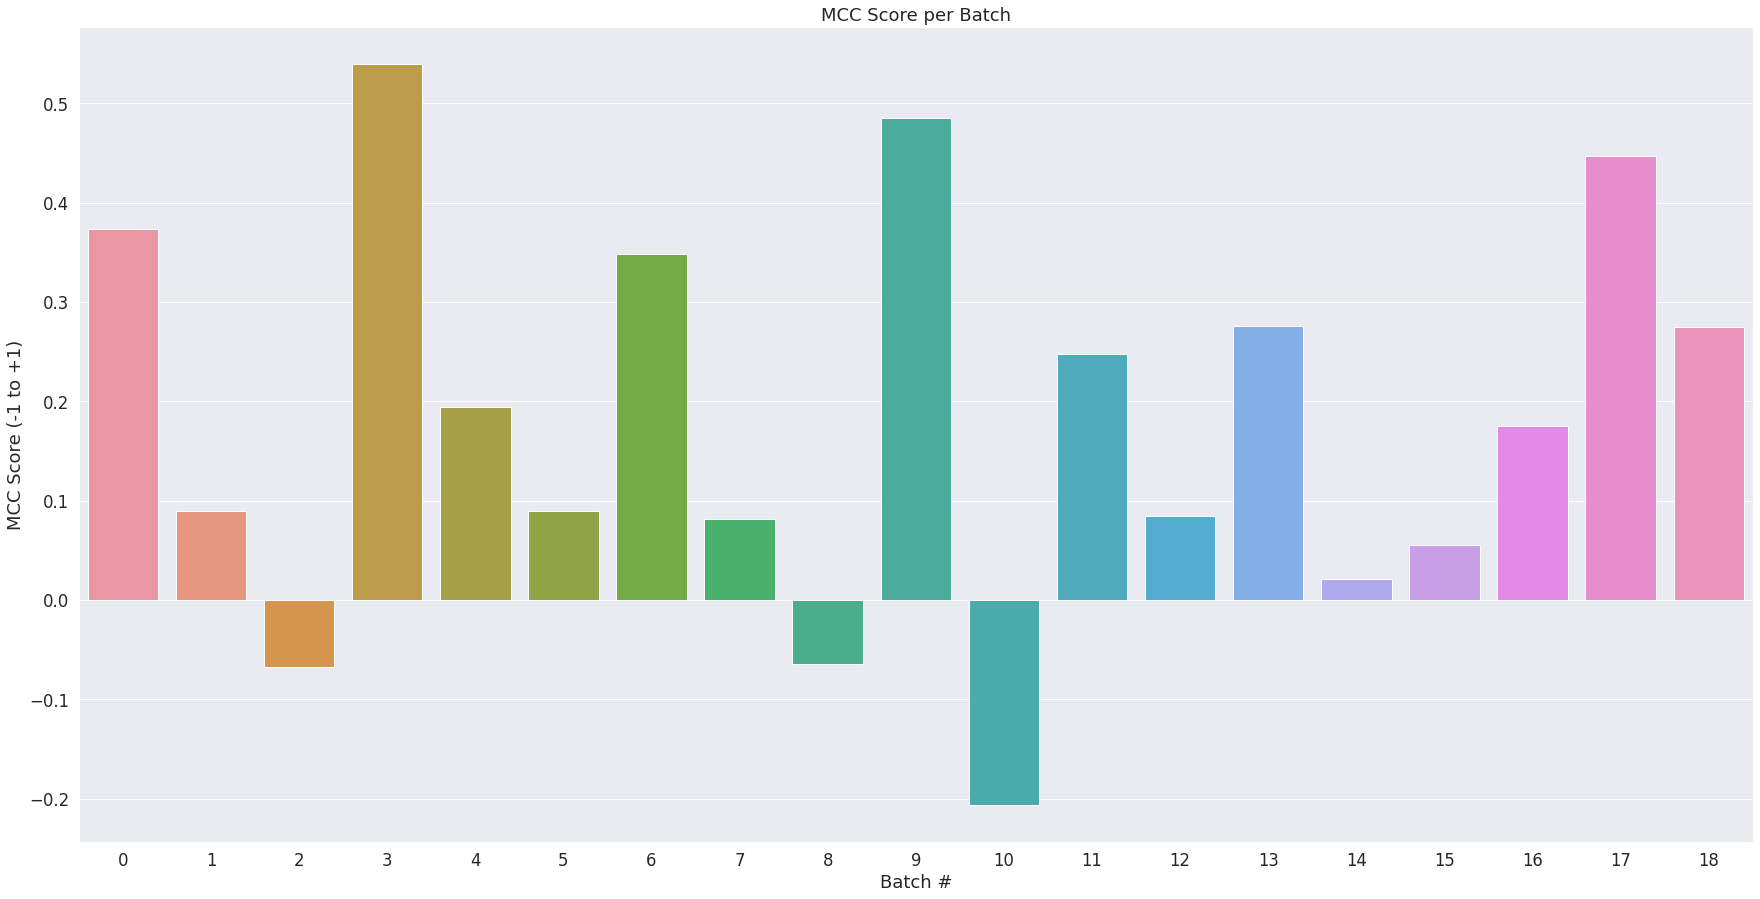
\includegraphics[width=8.5cm]{mcc.png}}
%  \vspace{2.0cm}
  \centerline{Fig. 1: MCC Score Per Batch for BERT}\medskip
\end{minipage}
%



\begin{minipage}[b]{1.0\linewidth}
  \centering
  \centerline{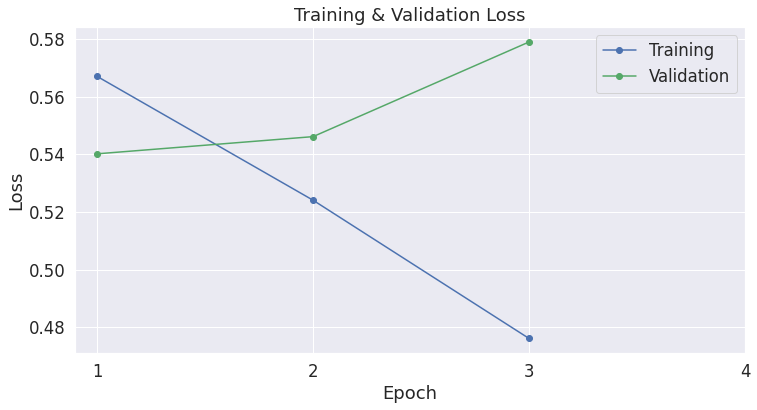
\includegraphics[width=8.5cm]{testvalid.png}}
%  \vspace{1.5cm}
  \centerline{Fig. 2: Test and Validation of BERT's Training}\medskip
\end{minipage}
\hfill

\end{figure}

{\rowcolors{1}{gray!30}{gray!20}
\begin{tabular}{ |p{3.5 cm}|p{3.5cm}|  }
\hline
\multicolumn{2}{|c|}{MCC Scores of Models} \\
\hline
Method & MCC \\
\hline
Sentiment Classification & -0.0027 \\
BERT & 0.152 \\
\hline
\end{tabular}
\centerline{ }

\centerline{Table 1: MCC scores from our Baseline and Bert}
}
\vspace{.5cm}

Our BERT model shows a very weak semantic evidence between viral and stumped tweets. 
Our model was slightly over-fit to the data trained as shown in figure 2 but overall it appears to be a well-trained model for our purposes. 
Any increase in epochs increased over-fitting by a huge rate to which the model was unusable and caused the MCC to be undefined at certain points of the graph.
We see that the MCC per batch (figure 1) is very scattered and in a few batches, we performed worse than guessing but most batches were classified better than guessing. 
Overall, the MCC over the batches was 0.154 so there is extremely weak semantic evidence that we can classify viral tweets and stumped tweets. 
The model, does however, outperform our baseline at a statistically significant rate which is better but not exceptional.

\subsection{Linguistic Tweet Evidence}
For reference, we have celebrity tweets that are $27\%$ popular and $73\%$ unpopular which is also the probability that they are chosen. 
This is important when we review our conditional probabilities. 
We consider anything drastic if the conditional probability is $\pm$10\%. 

\subsubsection{Emojis}

We determined if tweets had any of the currently recognized emojis located in the pip package \textit{emoji}. 
The conditional probabilities of viral and stumped that there are emojis are very similar to the proportions of popular and unpopular tweets which suggests that the existence of emojis does not affect how well a tweet performs since they are independent variables. \\

{\rowcolors{1}{gray!30}{gray!20}
\begin{tabular}{ |p{3.55 cm}|p{3.45cm}|  }
\hline
\multicolumn{2}{|c|}{Emoji Conditional Probabilities} \\
\hline
$P(X | Y)$ & Probability \\
\hline
$P(Viral | Emojis)$  & 28.5\% \\
$P(Stumped | Emojis)$ & 71.4\% \\
$P(Viral | No Emojis)$ & 27.0\% \% \\
$P(Stumped | No Emojis)$ & 73.0 \%  \\
\hline
\end{tabular}
\centerline{ }

\centerline{Table 2: Probabilities of Viral Tweets given Hashtags}
}

\subsubsection{Hashtags}

We determined if tweets had any hashtags to see if following trends increase the performance of tweets.
The conditional probabilities of viral and stumped tweets given the existence of a hashtag is located in table 3. 
Once again, we see that conditional probabilities given that there are hashtags or no hashtags are very similar to the proportions of popular and unpopular tweets.
This suggests that the existence of hashtags, or lack thereof, does not affect how well a tweet performs significantly enough and are independent variables.
In fact, if we consider $P(Stumped | Hashtag)$ to be significant, it is odd because usually users search for hashtags to read through. \\

{\rowcolors{1}{gray!30}{gray!20}
\begin{tabular}{ |p{3.7 cm}|p{3.3cm}|  }
\hline
\multicolumn{2}{|c|}{Hashtag Conditional Probabilities} \\
\hline
$P(X | Y)$ & Probability \\
\hline
$P(Viral | Hash)$  & 21.5\% \\
$P(Stumped | Hash)$ & 78.5\% \\
$P(Viral | No Hash)$ & 30.0\% \\
$P(Stumped | No Hash)$ & 70.0 \%  \\
\hline
\end{tabular}
\centerline{ }

\centerline{Table 3: Probabilities of Viral Tweets given Hashtags}
}

\subsubsection{Excessive Caps}

We used a threshold of 30\% of text in caps to classify excessive caps and classified no excessive caps for anything with less than 10 English letters in the text. 
We assumed that the tweets would get the attention of users if the conditional probabilities of viral and stumped tweets given the existence of excessive cap use is located in table 4. 
Once again, we see that conditional probabilities given that there are caps or no caps are very similar to the proportions of popular and unpopular tweets.
This suggests that the existence of caps, or lack thereof, does not affect how well a tweet performs significantly enough and thus independent variables. \\

{\rowcolors{1}{gray!30}{gray!20}
\begin{tabular}{ |p{3.5 cm}|p{3.5cm}|  }
\hline
\multicolumn{2}{|c|}{Caps Conditional Probabilities} \\
\hline
$P(X | Y)$ & Probability \\
\hline
$P(Viral | Caps)$  & 28.7\% \\
$P(Stumped | Caps)$ & 71.3\% \\
$P(Viral | No Caps)$ & 26.8\% \\
$P(Stumped | No Caps)$ & 73.2 \%  \\
\hline
\end{tabular}
\centerline{ }

\centerline{Table 4: Probabilities of Viral Tweets given Emojis}
}

\section{Discussion}
\label{sec:discussion}

All three of our approaches, sentiment classification, BERT, and linguistic evidence all produced evidence that suggests there is no relationship between sentiment, semantic, or linguistic cues and the performance of tweets.
Our sentiment classification was no better than guessing according to its MCC score. 
Our BERT model slightly performed better at our sentiment classification but still offered a very weak accuracy and weak evidence for a semantic relationship. 
Finally, our linguistic evidence showed that all three different cases produced no significant evidence for a linguistic evidence.

It may be possible to understand why this is possible due to our assumptions. 
Firstly, we used tweets from celebrities and the most followed accounts on Twitter. 
We assumed that this would be a good idea because they have the most engagement so it would be clear when a tweet outperforms the rest.
This also removes the randomness of our assessment to use statistical means to prove our findings and so we can only settle for evidence without statistical proof.
This may also be flawed due to different events such as the time of posting or controversies in the news which was not controlled for.
Moreover, it is possible that people do not read celebrity tweets and instead like to show support.

It is also possible that there was simply not enough tweets gathered. 
With 3,500 tweets from top followed accounts and a 600-less set to train BERT, it was possibly simply not enough to get any meaningful data out of it. However, we can suggest with our data that celebrities are adored and influence us. 
This evidence and observations gathered may show us that celebrities are considered different from regular users in how they are interacted with.

\section{Future Work}
\label{sec:future}

Our work produced a small amount of evidence that we can classify and predict if a tweet will be viral relative to a celebrity's following. 
However, we did not explore the chance of using a BERT model that was trained on tweets.
This would be a good future topic to explore to see if we can get a better BERT model with models trained on millions of tweets. 
Moreover, we acknowledge that our data was small. 
With Twitter making it difficult to obtain tweet data by making web-scraping difficult and putting all their APIs behind paywalls or throttling requests, it was difficult to obtain good data and as a result, we had to settle for a small amount of tweets. 
Another future work would be to use and collect much more tweet data, i.e. hundreds of thousands.
One other possible future work is to integrate every-day twitter users into this model instead of focusing on celebrities which can see if there is a relationship that does not exist with celebrities improving how we understand social influencers and their influence on us more concretely. 
We could also introduce a Coh-Metrix analysis of the texts to classify the writing styles of these texts. 
We could not in this paper since the website broke but this would be an excellent and more overhead approach than only approaching it with specific tweet features.
Lastly, an excellent future work would be to try this approach on another social media platform, such as Facebook, to determine if different social media platforms have different qualifications that make tweets perform better.

\bibliographystyle{IEEEbib}
\bibliography{strings,refs}

\appendix

\section{Contributions}

\begin{enumerate}
    \item Joshua Bugryn
    \begin{enumerate}
        \item Collected Tweet Data including getting through the hardships of Twitter's API
        \item Researched ways to classify BERT
        \item Researched different ways to obtain data from our texts
    \end{enumerate}

    \item Justin Sostre
    \begin{enumerate}
        \item Wrote BERT model training, testing, and ran.
        \item Wrote some of the report
        \item Developed Linguistic Evidence Testing
    \end{enumerate}
    
    \item Josh Wilson
    \begin{enumerate}
        \item Wrote and gave the project presentation
        \item Wrote first draft report
        \item Wrote some of final report
    \end{enumerate}
    
    \item All
    \begin{enumerate}
        \item Proof-read Report
        \item Collaborated on Demo and Project Presentation
    \end{enumerate}
\end{enumerate}

\end{document}
